This chapter introduces to essential topics and concepts in the context of this work and provides the reader with background knowledge required to follow in later chapters.

\section{Autonomous Driving}
\label{sec:background:autonomous_driving}
Academia and established industry leaders in automobile manufacturing are vigorously pushing research on autonomous driving technologies alongside emerging start-up companies, who try to enter the new market. The challenge of self-driving cars is believed to be solved within a few decades with high certainty \cite{Frost&SulivanConsulting2018}, although precise forecasts diverge. However, most experts agree that the benefits are enormous. Such include decreased risk of collisions and causalities, higher traffic efficiency and less occupied roads – leading to better environmental sustainability – and enhanced driver comfort. New business models – like robo-taxi- or car-sharing services – are likely to arise as transportation culture will undergo a shift from individually owned cars towards a sharing economy and \textit{Mobility as a Service} concepts. Nonetheless, despite these advantages, AD is also accompanied by a number of challenges. Most importantly, government regulations and an appropriate legal framework are vital. Moreover, people are commonly concerned about the accompanying loss of jobs and the cultural changes in general \cite{schoettle2014survey}. 

\subsection{Levels of Autonomy}
\label{subsec:background:labels_of_autonomy}
With reference to self-driving cars, a distinction is usually made between five different levels of autonomy \cite{Klein}. These levels are used to commonly describe vehicles' capabilities and their degree of independence from a human driver with regard to the task of driving. 

\begin{samepage}
\begin{itemize}
	\item \textbf{Level 0 ("'Active driver"'):} No computer assistance of any kind. A car is completely controlled by its human driver.
	\item \textbf{Level 1 ("'Feet off"'):} Basic assistance, e.g. adaptive cruise control. While most functions are controlled by the driver, the car might take responsibility of a single task, e.g. accelerating and decelerating in certain scenarios.
	\item \textbf{Level 2 ("'Hands off"'):} Partial automation, e.g. cruise control and lane centering. At this level, a car is able to take over multiple driving tasks in combination. While the driver is still required to monitor the roadway, she is "'disengaged from physically operating the vehicle"' \cite{Klein} and may keep her hands of the steering wheel and feet of the pedals. To ensure that a driver is still pays full attention and is able to intervene in case of system failures or critical situations, various methods of \textit{Driver Monitoring} are employed. Such include to visually observe a driver's face using cameras or to measure the force applied to the steering wheel.
	\item \textbf{Level 3 ("'Eyes off"'):} High degree of automation. At this level, a driver might fully rely on a car's self-driving under most conditions, delegating all safety-critical function to the ADAS. Usually, it would maintain a comprehensive awareness of its environment and is able to react on it. Although a driver still has to be present and prepared to take occasional control, she is not required to constantly monitor the traffic. 
	\item \textbf{Level 4 ("'Attention off"'):} Full automation. This refers to a system that is able to "'perform all safety-critical driving functions and monitor roadway conditions for an entire trip."' \cite{2016transportation} At this level, there is no necessity for a driver to actually occupy the vehicle.Driving performance of Level 4 autonomous cars is at least equal to human level and would generally even surpass it. 
	\item \textbf{Level 5 ("'Passive passenger"'):} Full autonomy. The highest level of automation describes a system that is capable of driving under any conditions, even extreme ones. Its performance is expected to be at least human-like or even surpass human driving capabilities. 
\end{itemize}
\end{samepage}


With this classification, it is worth noting that only the highest level actually refers to the term "'autonomy"'. \cite{wood2012potential} states that although this term is in more widespread public use, speaking of "'automation"' would be more accurate for levels 1 to 4. Only Level 5 cars are self-governing and may take independent decisions, e.g. selecting a destination and an appropriate route, while cars of all other levels still have a human person in the driver's seat.

\subsection{State of the Art}
\label{subsec:background:state_of_the_art}
Many of the major car brands have Level 2 vehicles in production today and some already offer models with experimental Level 3 technology \cite{Frost&SulivanConsulting2018}. One of the most famous examples is Tesla's AutoPilot \footnote{\url{https://www.tesla.com/autpilot}}, which is able to follow a route on the highway towards a given destination autonomously, while keeping and changing lanes on its own. According to \cite{Frost&SulivanConsulting2018}, \textit{"'China is expected to lead North America and Europe by the number of automated vehicles sold, whereas technology penetration wise, Europe is expected to lead the market for autonomous driving globally [by 2025]"'}. By 2015, 2 million Level 4 vehicles could be sold in Europe, while the first Level 5 vehicles could reach production readiness by 2030 \cite{McKinseyCenterforFutureMobility2019}. 

Market revenue for ADAS is expected to double by 2021 to reach \$35 million \cite{McKinseyCenterforFutureMobility2019}. Accordingly, many OEMs, including \textit{General Motors} and \textit{Volkswagen}, invest in acquiring AD start-up companies to extend their technological know-how to gain competitive advantages \cite{Korosec, Korosec2019}. In addition, big players from the tech industry push into the market with self-driving car fleets and shuttle services, including Uber \footnote{\url{https://www.uber.com}}, Lyft \footnote{\url{https://self-driving.lyft.com/}} and Waymo \footnote{\url{https://www.waymo.com/}}. 

On the technological side, hardware manufacturers like Nvidia \footnote{\url{https://developer.nvidia.com/drive}} and Qualcomm \footnote{\url{https://www.qualcomm.com/invention/5g/cellular-v2x}} invest in research on AD- and V2X-specific chips and machine learning hardware. Moreover, online education platforms like Coursera \footnote{\url{https://www.coursera.org/lecture/machine-learning/autonomous-driving-zYS8T}} and Udacity \footnote{\url{https://www.udacity.com/course/self-driving-car-engineer-nanodegree--nd013}} offer specific courses on AD to target the increasing demand for experts on these subjects. With Baidu Apollo \footnote{\url{https://github.com/ApolloAuto/apollo}} and Autoware.AI \footnote{\url{https://gitlab.com/autowarefoundation/autoware.ai}} there are even comprehensive, end-to-end AD platforms available as open-source software to be used in simulation or installed on a real car. 

\subsection{Sensor Fusion}
\label{subsec:background:sensor_fusion}
Additional sensors compared to non-autonomous cars are mainly required for two purposes: perception and localization. The former refers to the vehicle acquiring a detailed model of its surrounding, including type, position and speed of other traffic participants, traffic light state and more. The latter means to accurately find the vehicle's own position on a map. Current Level 2 vehicles already have a multitude of different sensors and \cite{Frost&SulivanConsulting2018} predict that future Level 5 cars might even have between 28 and 32 different sensors. 

\subsubsection{Sensors}
For \textbf{localization}, mainly GPS (Global Positioning System) and IMU (Inertial Measurement Unit) sensors are used. The latter usually consists of a combination of accelerometers and gyroscopes and helps to locate the vehicle even when no GPS connection is available. Occasionally, laser sensors (LiDAR) and radar technology are used in addition for more accurate positioning. While some approaches tend to rely on detailed, high-definition maps for even more precise positioning, others oppose the necessity of a car to know its position at centimeter-level accuracy \cite{Friedman2019}. When using high-precision sensory, the sole localization problem is often extended to \textit{Simultaneous Localization and Mapping} (SLAM).

For \textbf{perception}, most current approaches rely on (stereo) cameras, ultrasound sensors and radar. Some manufacturers consider LiDAR crucial in addition, while others, e.g. Tesla and Nissan \cite{McKinseyCenterforFutureMobility2019}, strictly oppose its use for perception or localization tasks. Comma.ai \footnote{\url{https://comma.ai}} even followed the approach of solely employing cameras for perception, arguing that, given the human example, decent driving performance can be achieved with only optical sensory. 

\subsubsection{Fusion}
\textbf{Sensor Fusion} \textit{"'is the combining of sensory data or data derived from sensory data such that the resulting information is in some sense better than would be possible when these sources were used individually"'} \cite{Elmenreich2002}. This also includes data normalization and temporal alignment.

\cite{Chen2019} differentiates between three levels (depicted in figure  \ref{fig:fusion_levels}) on which sensor fusion can happen, whereas the data subject to a fusion process is increasingly abstract at higher levels. 

\begin{figure}[H]
	\centering
	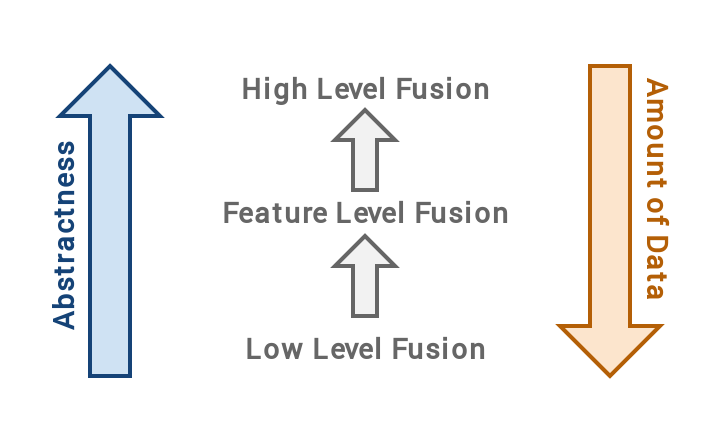
\includegraphics[width=0.5\textwidth]{98_images/fusion_levels.png}
	\caption{Levels of Sensor Fusion}
	\label{fig:fusion_levels}
\end{figure}

\begin{itemize}
	\item \textbf{Low Level Fusion:} Raw sensor data is subject to the fusion process. Input might be LiDAR point clouds, RGB camera images, etc. Commonly used algorithms are Kalman filters, Bayesian networks and, more recently, also Neural networks.
	\item \textbf{Feature Level Fusion:} Before fusion, certain features are extracted from the raw data. For instance, if some component within the AD stack is responsible for lane keeping, lane markings could be extracted from raw RGB images for this purpose, e.g. using a Canny filter. Input might either be raw sensor data or the outputs from a subsequent low-level fusion step.
	\item \textbf{High Level Fusion:} High-level operates on the level of objects, which are extracted from sensor data. In the context of Cooperative Perception these objects might usually be other traffic participants with their respective properties. Input will usually be the outputs of some form of subsequent low- or feature-level fusion.
\end{itemize}

As explained in greater detail in later chapters, this work will mostly deal with high-/object-level fusion. 


\subsection{Autonomous Driving Pipeline}
\label{subsec:background:autonomous_driving_pipeline}

\begin{figure}[H]
	\centering
	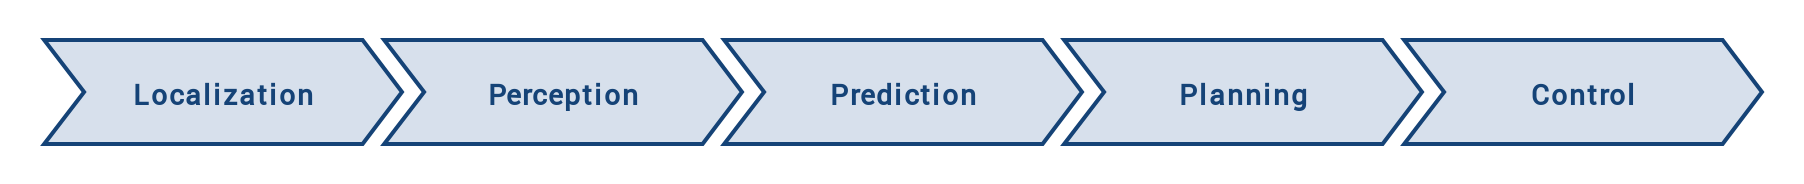
\includegraphics[width=\textwidth]{98_images/ad_pipeline.png}
	\caption{Autonomous Driving Pipeline}
	\label{fig:autonomous_driving_pipeline}
\end{figure}

The process from sensing the environment to controlling a self-driving car can be categorized into steps of a pipeline, that is repeatedly run. 

\begin{enumerate}
	\item \textbf{Localization:} Often implemented as a combined \textit{Simultaneous Localization and Mapping} (SLAM) problem, goal is to determine the vehicle's current position on a map with high precision. Common algorithms and sensors used in this step were described in \ref{subsec:background:sensor_fusion}.
	\item \textbf{Perception:} A crucial step towards AD is to perceive a vehicle's current environment, where perception is defined as the \textit{"'process of maintaining an internal description of the external environment"'} \cite{Crowley1993}. That includes to recognize, classify and locate other traffic participants and their static and dynamic properties as well as any other surrounding obstacles. In this thesis, the perception step is of primary interest. Common algorithms and sensors used in this step were described in \ref{subsec:background:sensor_fusion}.
	\item \textbf{Prediction:} Prediction builds on the outcome of the subsequent perception step and aims to estimate a future state $\hat{\theta}\textsubscript{t+1}$ of the vehicle's surrounding environment, given an observation $\theta\textsubscript{t}$ at present time. For instance, the future trajectory of a nearby car might be approximated. The problem of \textbf{tracking} objects over multiple frames / multiple, repeated executions of the AD pipeline can also be considered part of the prediction step. 
	\item \textbf{Planning:} Given the vehicle's own current position as well as estimations for the future state of all other nearby traffic participants, the planning step aims to find an appropriate trajectory that satisfies certain requirements and minimizes a given cost metrics. For instance, given a global target position, a collision-free trajectory might be found that is physically feasible, compliant with traffic rules, minimizes \textit{jerk} (the accumulated magnitude of the acceleration change \cite{paden2016survey}), a maximizes the average distance to all obstacles. Planning can be divided into the sub problems of \textbf{(1) Routing}, \textbf{(2) Behavior Planning} (e.g. choose an action $a \in \{ "'keep\_lane"', "'change\_lane"', "'stop"', "'accelerate"', ... \}$) and \textbf{(3) Motion Planning}. (3) again, usually is solved in two steps, namely (3.1) Path Planning and (3.2) Trajectory Planning. (3.1) is considered to be PSPACE-complete \cite{paden2016survey}. Commonly used algorithms include, but are not limited to A* and RRT*.
	\item \textbf{Control:} Eventually, planning output needs to be translated into actual brake- throttle- and steering commands to physically control the vehicle through its actuators. 
\end{enumerate}

\section{Vehicle-to-X Communication}
\label{sec:background:v2x_communication}
Vehicle-to-X, or Vehicle-to-Everything, communication generally describes the Internet Of Things (IoT) approach of having (autonomous) vehicles exchange information with other actors in their local environment through messaging.

\subsection{Application Types}
\label{subsec:background:application_types}
A V2X communication system can have different constellations, depending on what participants are involved.

\begin{itemize}
	\item \textbf{Vehicle-to-Vehicle (V2V):} The ability of cars to communicate with each other. This is among the most common instantiations of Vehicle-to-Everything communication. 
	\item  \textbf{Vehicle-to-Infrastructure (V2I):} The ability to cars to communicate with any type of traffic infrastructure. Most commonly, vehicles bilaterally exchange information with traffic lights to optimize traffic flow. Further examples include automated fare collection or emergency vehicles path cleaning.
	\item \textbf{Vehicle-to-Pedestrian (V2P):} The ability of cars to indirectly communicate with nearby pedestrians, mainly used to prevent collision. Pedestrians need to be equipped with smartphones or wearable devices to take part in the communication.
	\item \textbf{Vehicle-to-Grid (V2G):} The ability of cars to communicate with entities of the electrical power grid. With this approach, \textit{"'[...] plug-in electric vehicles, such as battery electric vehicles (BEV), plug-in hybrids (PHEV) or hydrogen fuel cell electric vehicles (FCEV), communicate with the power grid to sell demand response services by either returning electricity to the grid or by throttling their charging rate."'} \cite{wiki:v2g}
	\item \textbf{Vehicle-to-Cloud (V2C):} The ability of cars to communicate with all kinds of cloud services, e.g. to get real-time traffic information, find parking spots, receive over-the-air software updates from its vendor or consume multi-media entertainment.
\end{itemize}

Especially V2I and V2G patterns will likely emerge as "'Smart Cities"' establish in the near future.

This thesis mainly addresses V2V and V2I use cases.

\subsection{Communication}
\label{subsec:background:communication}
There are two types of V2X communication technology depending on the underlying technology being used, namely \textit{Dedicated Short-Range Communications} (DSRC) and Cellular-V2X (C-V2X)-based approaches. Each of them imply different communication patterns.

Today, DSRC is more common. It usually relies on WiFi-based communication using the IEEE 802.11p standard and implies \textit{Vehicular Ad-Hoc Networks} (VANETs) as communication topology. In the case of VANETs, vehicles and infrastructure devices (or road-units (RSUs)) in range form pairwise connections among each other and build up a peer-to-peer (P2P) network. Besides direct message exchange, VANETs usually also support multi-hop communication to reach out to further distant actors beyond WiFi range and line-of-sight. The European version of DSRC, standardized by CEN \footnote{\url{https://www.cen.eu}}, is also referred to as ITS-G5 to avoid confusion. 

In 2016, a first specification of C-V2X technology using Long-Term Evolution (LTE) networks was published by 3GPP \footnote{\url{https://www.3gpp.org}}. Especially with the upcoming establishment of 5G networks, C-V2X is becoming increasingly attractive as dramatically improved latency and throughput allow for high-performance applications. With C-V2X, both P2P-based- as well as centralized, wide-area communication are possible. 

\section{Cooperative Perception}
\label{sec:background:cooperative_perception}

\subsection{Concept \& Motivation}
\label{subsec:background:concept_motivation}
Although perception accuracy and reliability have greatly improved over time, current systems still fail to completely comprehend complex situations occasionally. This may lead to incorrect decisions and potentially to collisions. Consequently, relying on local sensors only is insufficient under certain circumstances, especially in situations with very limited line-of-sight (LOS).

Using V2X communication, next generation vehicles might be able to extend their perception range vastly. More precisely, they might be enabled to exchange information about their own state in combination with sensor data or a higher-level local environment model. Connected cars could become an additional, virtual sensor to each other. Accordingly, cooperative (or collective) perception can be viewed as a sensor fusion problem, whereas a "'cooperative"' sensor network is characterized as such that \textit{"'[...] uses the information provided by two independent sensors to derive information that would not be available from the single sensors."'} \cite{Elmenreich2002}. The different fusion levels introduced in chapter \ref{subsec:background:sensor_fusion} apply analogously with respect to the data being shared among CP-enabled vehicles (e.g. raw sensor measurements or high-level objects).

However, as already found by \cite{Gunther2015}, a drawback of CP – as with any other system relying on the presence of a network – is the network effect: a CP system is only useful once the number of participants exceeds a certain critical mass. Accordingly, for CP to succeed, it is crucial to follow a rather aggressive market penetration strategy during its introduction. Preferably, different OEMs would collaborate to build one unified system.

\subsection{Use Cases}
\label{subsec:background:use_cases}
Cooperative Perception is expected to bring two essential improvements. First, vehicles' field-of-view is extended virtually (\textbf{Non Line-of-Sight Sensing [NLOS]}). Second, \textbf{confidence} for observations within an area, that is overlapped by the perception range of two or more connected cars, can be improved through "'voting"'.

\begin{figure}[h]
	
	\begin{subfigure}{0.5\textwidth}
		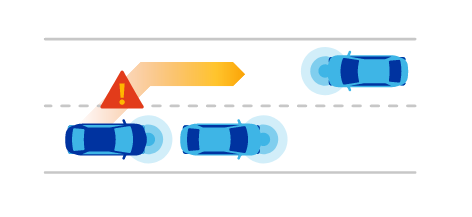
\includegraphics[width=1.0\linewidth, height=5cm]{98_images/nloss_2.png} 
		\caption{Opposing traffic out of sight}
		\label{fig:cp_use_cases_1}
	\end{subfigure}
	\begin{subfigure}{0.5\textwidth}
		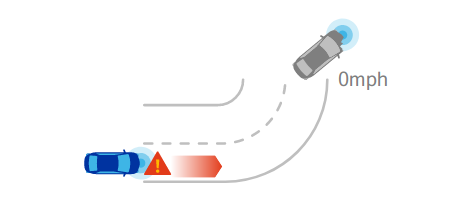
\includegraphics[width=1.2\linewidth, height=5cm]{98_images/nloss_3.png}
		\caption{Vehicle behind a curve}
		\label{fig:cp_use_cases_2}
	\end{subfigure}
	
	\caption{Exemplary non line-of-sight scenes (source: \cite{QualcommTechnologiesInc.2017})}
	\label{fig:cp_use_cases}
\end{figure}

Figure \ref{fig:cp_use_cases} depicts two traffic situations in which CP can greatly help to improve safety. In scene \ref{fig:cp_use_cases_1}, the leftmost vehicle is about to overtake, but cannot see the opposing traffic, because its sight is restricted by the vehicle in front. However, since both other cars are broadcasting their own state and their perceptions, it is virtually moved into range of sight. Similarly, in \ref{fig:cp_use_cases_2}, the blue could can only recognize the stopped car once it has already passed the curve and might have do brake sharply without CP

\section{Edge Computing}
\label{sec:background:edge_computing}

\begin{figure}
	\centering
	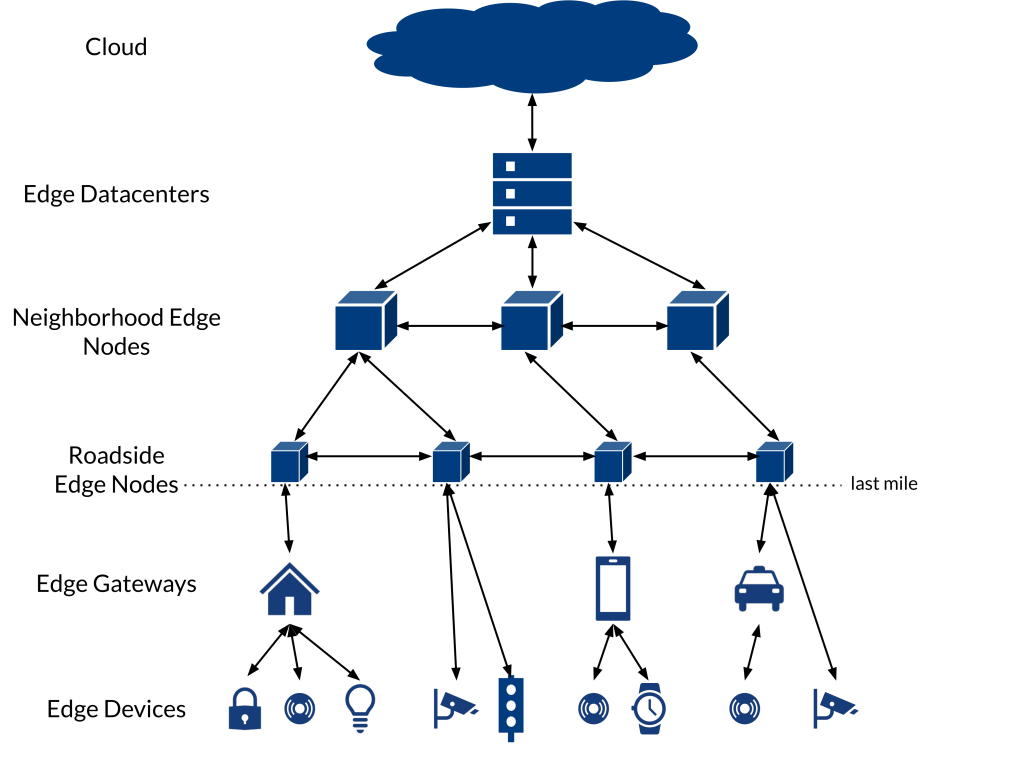
\includegraphics[width=0.8\textwidth]{98_images/edge.png}
	\caption{Architecture of Edge Computing (source: \cite{Bischoff2019})}
	\label{fig:edge_computing}
\end{figure}

Edge computing is an architecture design pattern for distributed software applications. \textit{"'In general, [it] [...] is the process of performing computing tasks physically close to target devices, rather than in the cloud or on the device itself"'} \cite{Bischoff2019}. Usually, one or more additional layers of computation devices (edge nodes, edge gateways) are introduced as intermediate "'hops"' between end-device and the cloud. This is especially beneficial in IoT contexts, where devices are comparatively weak in terms of computational capabilities, while the amounts of gathered data can quickly become huge. Accordingly, on the one hand, high load is taken from those low-power devices and, on the other hand, latency between device and analytics server is kept small. In the context of Cooperative Perception, low latency is especially crucial, so edge computing appears to be a promising pattern.

Besides having stronger hardware (and therefore higher \textbf{compute capacity}) for data processing tasks compared to the end-devices themselves and better \textbf{latency} compared to using cloud infrastructure, edge computing comes with additional advantages. Through a higher degree of distribution \textbf{reliability}, \textbf{scalability} and \textbf{robustness} can be improved. Moreover, by employing edge servers, \textbf{costs} can be reduced and \textbf{security} can be increased, especially when dealing with privacy-sensitive applications and data. 

Recently, another term for a similar concept has established: \textbf{fog computing}. While boundaries between edge- and fog computing are blurry, one could argue that fog nodes could make up an additional layer of abstraction and are placed between edge- and cloud nodes. In the example of a large IoT-enabled factory, edge nodes could exist within the local area network of each shop floor, while one or more fog nodes are located in a company-internal micro data center. Both of them would usually have the task to analyze and process data from the previous step to pre-process, filter and summarize it before it eventually gets send into the cloud.

In the context if this thesis, an additional layer of indirection is not considered necessarily and, therefore, the terms are used interchangeably for the sake of simplicity. 

\section{Geo Tiling}
\label{sec:background:geo_tiling}
Geo tiling, or \textit{hierarchical binning}, is a strategy to represent, uniquely identify and index geospatial data. The idea is to \textit{"'store a geo-database such that data for a specific location can be retrieved quickly, by dividing the data up by location, partitioning the world into tiles"'} \cite{wiki:quadtiles}. 

\subsection{QuadKeys}
\label{subsec:background:quadkeys}

\begin{figure}[H]
	\centering
	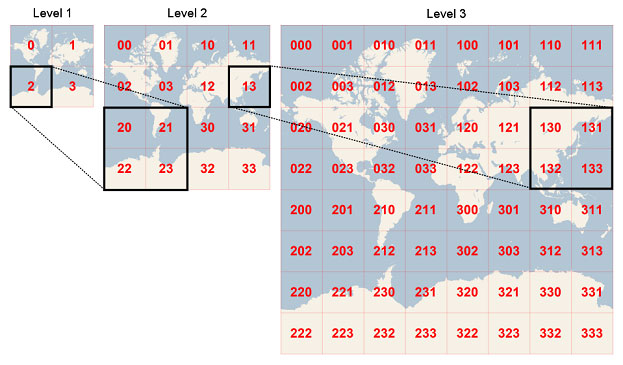
\includegraphics[width=0.8\textwidth]{98_images/quadkeys.jpg}
	\caption{Geo tiling with QuadKeys (source: \cite{wiki:quadtiles})}
	\label{fig:quadkeys}
\end{figure}


One implementation of geo tiling is \textit{QuadKeys}, proposed by \cite{Schwartz2018}. Its idea is to recursively split the two-dimensional \textit{Mercator projection} of the world map into four square tiles. Assuming an earth circumference of 40,000 km, each of these tiles would be approximately 20,000 by 20,000 km in size at the first level. Each of these tiles is split into four tiles again, while the size of the tiles is halved in every iteration. Continuing this way, arbitrary precision can be reached in theory.

As depicted in figure \ref{fig:quadkeys}, every tile is uniquely identifiable by a number (or a text string) when enumerated recursively. The length of that string, and therefore the maximum spatial precision, is only limited by the size of the data types used during its calculation. When using 64-bit float variables, the maximum level is 54. At level 30, for instance, ground resolution at the equator is already 3.7 cm², while at level 54 it is 2.22*10\textsuperscript{-9} cm².

As an alternative to representing a QuadKey as a string, where, in case of using ASCII encoding, every character would be one byte in size, QuadKeys can also be represented as integers for better space efficiency. In integer representation, the length of a key is limited by the underlying data type (usually 64 bits). The size complexity is then given as $O(1)$ compared to $O(n)$ with strings ($n$ being the precision level, or key length).

\par
\bigskip

In the course if this thesis, QuadKeys are used to uniquely and uniformly reference geographical locations. 